\chapter{State of the Art}
\label{cap:estadoDeLaCuestion}

\section{Gmail API}\label{sect:gmailapi}
In order to be able to read and send emails, it is necessary to access to the user's email data. For this reason, the different ways to obtain this information were studied. One of them is the Gmail API, which allows developers to perform all the actions we need in an easy way.

Gmail API can be used in several programming languages such as Python, PHP, Go, Java, .NET, \ldots Due to the greater number of examples in the starting guides of the Gmail API \citep{gmailAPI} and the previous knowledge that was already had of it, Python was chosen for the first contact with this implement.

The following is a step-by-step explanation of what is necessary to do to access the user's Gmail account, create a message, send an email previously created, create and update a draft, reply a received message (for this it is necessary to know how to create an email) and read important information of message threads and individual emails (such as who is the sender, who will received the message, the subject, the date, the email's body, the attached files, \ldots).

\subsection{OAuth 2.0 Protocol}\label{ssect:oauth}
Gmail API, as it also happens in the case of other Google APIs, uses OAuth 2.0 protocol \citep{oauth} to handle authentication and authorization. As it will be seen later in this section, it is needed to be in possession of OAuth 2.0 client credentials from the Google API Console for having the appropriate permissions to use the Gmail API.

The Google API Console, also known as Google Console Developer\footnote{\url{https://console.developers.google.com/}}, built into Google Cloud Platform, makes possible an authorized access to a user's Gmail data. In order to achieve it, having a Google account is a prerequisite because it will be necessary to access to this platform. Once this web has been accessed, at first we have to create a new development project by clicking in ``New Project'' in the control panel (which is the main tab of the Google Console Developer and the one that opens by default when you access it). When we have already created a project, we will enable the API we are going to work with, in this case the Gmail API. To do this we will look for it in the search engine that we can find in the library of APIs of this platform. Now we can apply for the credentials we need. Accessing to the ``Credentials'' tab and clicking on ``Create Credentials'' will lead us to an easy questionnaire about what type of credentials we prefer that we have to answer by basing on what type of application we are building. Then we must download the .json file and save it in the folder we are going to work in.

Before starting the development of the implementation of the OAuth 2.0 protocol which will provides us a secure and trusted login system to access to the user's Gmail data, we must install the Google Client Library\footnote{\url{https://developers.google.com/gmail/api/downloads}} of our choice of language (as we have said we will use Python for this, so we have to install the libraries \textit{google-api-python-client}, \textit{google-auth-httplib2} and \textit{google-auth-oauthlib}).

There are many ways to obtain the necessary permissions for accessing to the user's emails data following the OAuth 2.0 protocol. As this is a first contact with the Gmail API only with the intention of knowing the possibilities it offers to us and its advantages and disadvantages of using it in our future implementation of our virtual assistant, we are going to develop a simple script which is using a class very useful for local development and applications that are installed on a desktop operating system. The class \textit{InstalledAppFlow}, in \textit{google\_auth\_oauthlib.flow} \citep{oauthlib}, is a \textit{Flow} subclass (which belongs to the same library). Thanks to this last class we have mentioned, \textit{InstalledAppFlow} uses a \textit{requests\_oauthlib.OAuth2Session} instance at \textit{oauth2session} to perform all of the OAuth 2.0 logic. Besides it also inherits from \textit{Flow} the class method \textit{from\_client\_secrets\_file} which creates a \textit{Flow} instance from a Google client secrets file (this file will be the .json file that we obtained through the Google API Console) and a list of OAuth 2.0 Scopes \citep{oauth-scopes}, which are a mechanism  in OAuth 2.0 to limit an application's access to a user's account. An application can request one or more scopes, this information is then presented to the user in the consent screen, and the access token issued to the application will be limited to the scopes granted (we will use the Gmail API OAuth 2.0 Scope which allows us to read, compose, send, and permanently delete all your email).

\begin{figure}[h]
	\centering%
	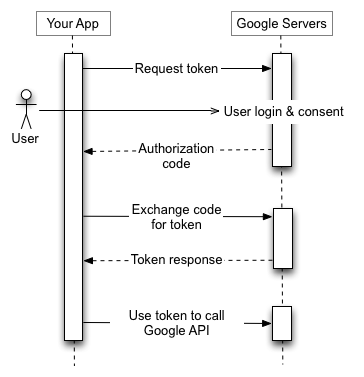
\includegraphics[width = 0.5\textwidth]{Imagenes/Bitmap/webflow.png}%
	\caption{OAuth 2.0 for Web Server Applications and Installed Applications.}%
	Image extracted from \cite{oauth}
	\label{fig:oauth}
\end{figure}

After constructing an \textit{InstalledAppFlow} by calling \textit{from\_client\_secrets\_file} as we have explained, we can invoke the class method \textit{run\_local\_server} which instructs the user to open the authorization URL in the browser and will attempt to automatically open it. This function will start a local web server to listen for the authorization response. Once there is a reply, the authorization server will redirect the user's browser to the local web server. As we can see in \ref{fig:oauth}, the web server will get the authorization code from the response and shutdown, that code is then exchanged for a token.

Then, we will be in possession of the OAuth 2.0 credentials for the user \citep{oauth2.credentials} which we are going to use for accessing the user's Gmail account. In summary, it is possible to obtain the necessary permissions from the user and to follow the OAuth 2.0 protocol, by executing these instructions (written in Python):

\begin{python}
from google_auth_oauthlib.flow import InstalledAppFlow

# Create a flow instance
flow = InstalledAppFlow.from_client_secrets_file('credentials.json', 
	['https://mail.google.com/'])
# Obtain OAuth 2.0 credentials for the user
creds = flow.run_local_server(port = 0)
\end{python}

Now, we are able to call Gmail API by using the token (which is stored in the variable \textit{creds}). However, before starting working on the email data, we should save the OAuth 2.0 credentials since otherwise the user would need to go through the consent screen every time the application is opened. To prevent the latter from happening, to differentiate access from mail management and consequently to reuse as much code as possible; we have implemented the following class \textit{auth}, in \textit{auth.py}, with a main method \textit{get\_credentials}:

\begin{pythonnum}
import pickle
import os.path
from google_auth_oauthlib.flow import InstalledAppFlow
from google.auth.transport.requests import Request
	
class auth:
	def __init__(self, SCOPES, CLIENT_SECRET_FILE):
		self.SCOPES = SCOPES
		self.CLIENT_SECRET_FILE = CLIENT_SECRET_FILE
	
	def get_credentials(self):
		"""
		Obtains valid credentials for accessing Gmail API
		"""
		creds = None
		# The file token.pickle stores the user's access and refresh tokens
		if os.path.exists('token.pickle'):
			with open('token.pickle', 'rb') as token:
				creds = pickle.load(token)
		# If there are no (valid) credentials available, let the user log in
		if not creds or not creds.valid:
			if creds and creds.expired and creds.refresh_token:
				creds.refresh(Request())
			else:
				flow = InstalledAppFlow.from_client_secrets_file(
					self.CLIENT_SECRET_FILE, self.SCOPES)
				creds = flow.run_local_server(port=0)
			# Create token.pickle and save the credentials for the next run
			with open('token.pickle', 'wb') as token:
				pickle.dump(creds, token)
		return creds

\end{pythonnum}

As we can observe in line 17 within \textit{get\_credentials} method, at first we check if the file called \textit{token.pickle} exists, and in that case, it is opened and its information is stored in the variable \textit{creds}. Thus, we avoid to force the user to open the authorization screen. By contrast, as we have seen before, if it does not exists, we obtain the credentials by calling the class methods \textit{from\_client\_secrets\_file} and \textit{run\_local\_server} (it is written between lines 25 and 30).

There is another case that is also reflected in the code above (in lines 23 and 24): the credentials are expired (it is possible to check it by executing \textit{creds.expired}) and they can be refreshed (the OAuth 2.0 refresh token is \textit{creds.refresh\_token}) \citep{oauth2.credentials}. In this situation, we will refresh the access token by invoking the method known as \textit{refresh} and by giving it a \textit{Request} object \citep{request-lib} from \textit{google.auth.transport.requests} as the function parameter which used to make HTTP requests.

\subsection{Building a Gmail Resource}
At this point, with the OAuth 2.0 credentials, we are able to call the Gmail API. For this purpose, it is necessary to construct a resource \citep[/v1/reference]{gmailAPI} for interacting with the API. The \textit{build} method, from \textit{googleapiclient.discovery} library \citep{build-module}, create that object. As we will see later, this resource will lead us to manage emails, drafts, threads and everything we will like to do with the user's Gmail data. This is why, using the \textit{auth.py} file explained in \ref{ssect:oauth}, we are going to start every user session with the instructions below (or their equivalents in the language we are using):

\begin{python}
from googleapiclient.discovery import build
import auth

SCOPES = ['https://mail.google.com/']
CLIENT_SECRET_FILE = 'credentials.json'

# Creation of an auth instance
authInst = auth.auth(SCOPES, CLIENT_SECRET_FILE)
# Constructing the resource API object
service = build('gmail', 'v1', credentials = authInst.get_credentials())
\end{python}

Henceforth, we will use the \textit{service} variable to relate it with the resource object created by the \textit{build} method.

\subsection{Messages resource}
In most of the operations we are going to execute, it will be essential the correct management of messages. Therefore, knowing how the emails are represented in Gmail API and how to use them is imperative to understand how to work with this API. For this reason, in this section we are going to delve into the \textit{Message} resource of the Gmail API, its structure and its methods.

Regardless of which programming language is used, \textit{Message} resource \citep[/v1/reference/users/messages]{gmailAPI} internally has a dictionary structure. The more important (for us) keys of this data structure are (at least the most useful keys for our purpose):
\begin{itemize}
	\item\textit{id}: an immutable string which identifies the message.
	\item\textit{threadId}: we will explain the thread resource in \ref{ssect:threads} and we will see that a thread is composed of different messages that share common characteristics. The value of this field is a string which represent the id of the thread the message belongs to.
\end{itemize}

\subsection{Threads resource}\label{ssect:threads}